\documentclass[pdftex,cig,slideColor]{pp4slides}
\usepackage{amsmath}
\usepackage{mpmulti}
\usepackage{multirow}
\usepackage{amsfonts}
\usepackage{pifont}
\usepackage{rotating} % use turn environment

\title{PyLith 1.0}
\subtitle{}
\author{Brad Aagaard, Charles Williams, Matthew Knepley\\[10pt]
  Sue Kientz and Leif Strand}
\institution{\includegraphics[height=2cm]{logos/CIG}}
\date{June 25, 2007}

% --------------------------------------------------------- DOCUMENT
\begin{document}

% ------------------------------------------------------------ SLIDE
\maketitle
\vfill

% ------------------------------------------------------------ SLIDE
\foilhead{Outline}
  \summary{}  

  \begin{itemize}
  \item Introduction to PyLith
    \begin{itemize}
    \item Motivation \& development objective
    \item What does PyLith do?
    \end{itemize}
  \item PyLith Design
    \begin{itemize}
    \item Architecture and programming languages
    \item Development strategy
    \end{itemize}
  \item Features
    \begin{itemize}
    \item Current release
    \item Planned releases
    \end{itemize}
  \item Example
  \item Feedback
  \end{itemize}

\bgadd{\vspace*{7.9in}%
  \begin{center}%
    
\includegraphics[height=14mm]{logos/cig}
  \end{center}}

% ------------------------------------------------------------ SLIDE
\foilhead{Motivation for Developing PyLith}
  \summary{}
  
  \begin{itemize}
  \item Available modeling codes
    \begin{itemize}
    \item rarely solve the problem {\bf you} want to solve
    \item are often poorly documented
    \item may not work correctly
    \end{itemize}
  \item Current research demands larger, more complex simulations
  \item Want to avoid multiple, incompatible versions of the same code
  \end{itemize}

% ------------------------------------------------------------ SLIDE
\foilhead{PyLith 1.0 Design Objective}
  \summary{Want to a code developed for and by the community}
  
  \begin{itemize}
  \item Modular
    \begin{itemize}
    \item Users can swap modules to run the problem of interest
    \end{itemize}
  \item Scalable
    \begin{itemize}
    \item Code runs on one to a thousand processors efficiently
    \end{itemize}    
  \item Extensible
    \begin{itemize}
    \item Expert users can add functionality to solve their problem
      without polluting main code
    \end{itemize}
  \end{itemize}

% ------------------------------------------------------------ SLIDE
\foilhead{PyLith 1.0}
  \summary{What is it good for?}

  \begin{itemize}
  \item Quasi-static crustal deformation
    \begin{itemize}
    \item Interseismic deformation
    \item Post-seismic deformation
    \item Volcano deformation
    \end{itemize}
  \item Dynamic rupture and wave propagation
    \begin{itemize}
    \item Kinematic (prescribed) earthquake ruptures
    \item Strong ground motion modeling
    \end{itemize}
  \end{itemize}

% ------------------------------------------------------------ SLIDE
\foilhead{PyLith 1.0}
  \summary{Overview of workflow for typical research problem}

  \vfill
  \begin{center}
    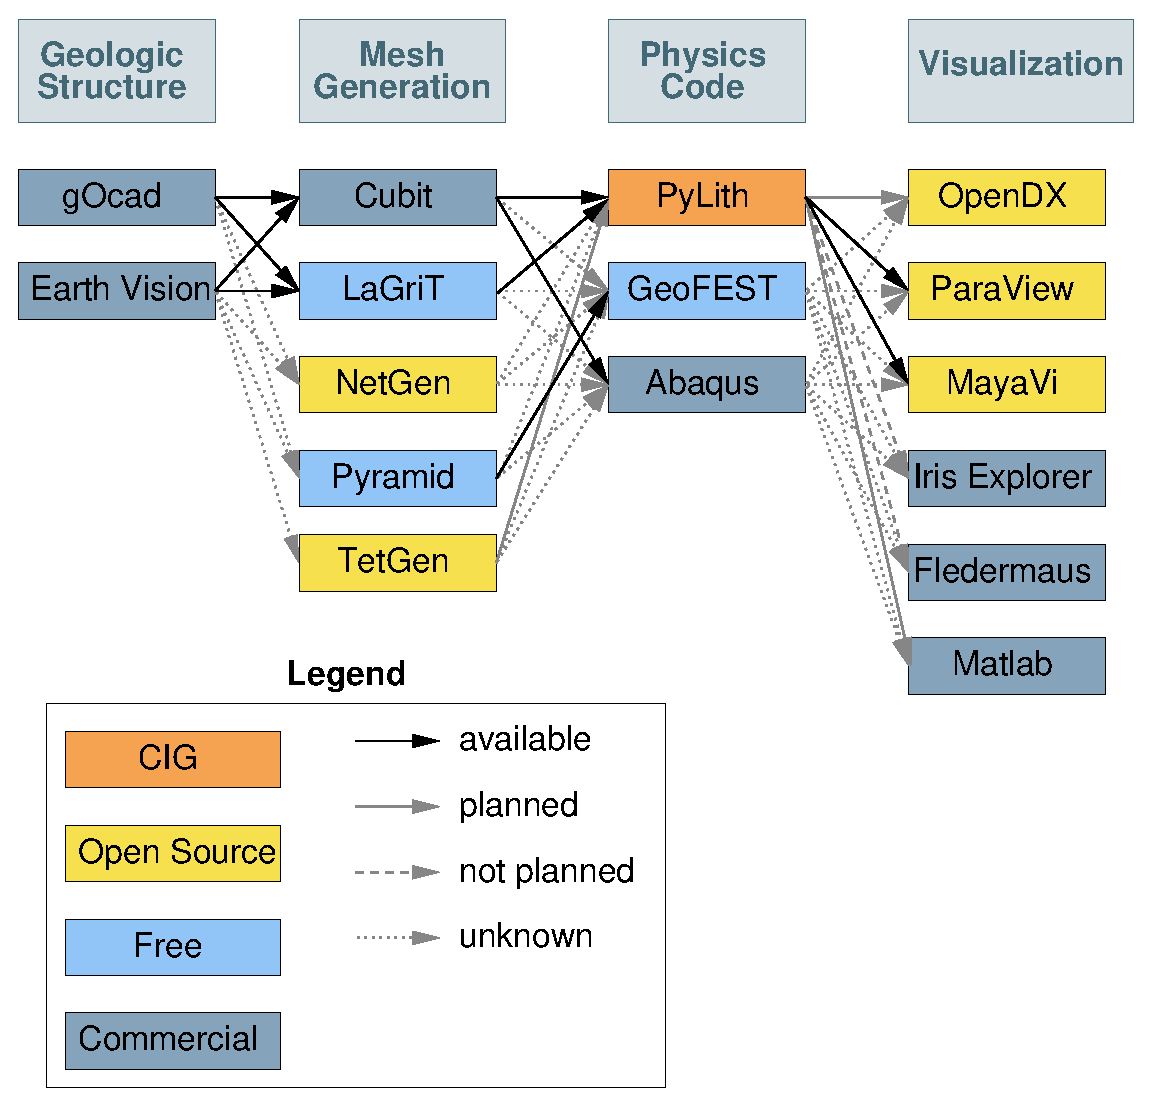
\includegraphics[scale=0.8]{figs/workflow}
  \end{center}

% ------------------------------------------------------------ SLIDE
\foilhead{PyLith Design: Focus on Geodynamics}
  \summary{Leverage packages developed by computational scientists}

  \vfill
  \begin{center}
    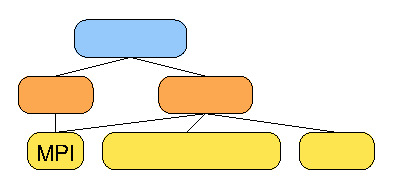
\includegraphics[scale=1.7]{figs/packages}
  \end{center}

% ------------------------------------------------------------ SLIDE
\foilhead{PyLith Design: Code Architecture}
  \summary{Flexible and modular with good performance}

  \begin{itemize}
  \item Top-level code written in Python
    \begin{itemize}
    \item Expressive, high-level,, object-oriented language
    \item Dynamic typing allows adding additional modules at runtime
    \item Convenient scripting
    \end{itemize}
  \item Low-level code written in C++
    \begin{itemize}
    \item Compiled (fast execution), object oriented language
    \end{itemize}
  \item Bindings to glue Python \& C++ together
    \begin{itemize}
    \item Pyrex/pyrexembed generate C code for calling C++ from Python
    \end{itemize}
  \end{itemize}

% ------------------------------------------------------------ SLIDE
\foilhead{PyLith Design}
 \summary{Tests, tests, and more tests ($>$500 in all)}
 
 \begin{itemize}
 \item Create tests for nearly every function during development
   \begin{itemize}
   \item Remove most bugs during initial implementation
   \item Isolate and expose bugs at origin
   \end{itemize}
 \item Create new tests to expose bugs reported
   \begin{itemize}
   \item Fast isolation of origin of bugs
   \item Prevent bugs from reoccurring
   \end{itemize}
 \item Rerun tests whenever code is changed
   \begin{itemize}
   \item Allows optimization of performance with quality control
   \item Code continually improves
   \end{itemize}
 \end{itemize}
  
% ------------------------------------------------------------ SLIDE
\foilhead{PyLith 1.0: Features}
  \summary{}

  \begin{itemize}
  \item User-interface
    \begin{itemize}
    \item Import meshes directly from LaGriT and CUBIT
    \item Easy specification of parameters for boundary condition and
      fault conditions
    \end{itemize}
  \item Applications
    \begin{itemize}
    \item Quasi-static solution of tectonic deformation
    \item Dynamic solution of wave propagation for propagating ruptures
    \end{itemize}
  \item Under the hood
    \begin{itemize}
    \item Sieve - parallel data structures for storing and
      manipulating finite-element meshes
    \item PETSc - large library of solvers and preconditioners
    \item Pyre - science neutral simulation framework for easy access
      to user data and configuration
    \end{itemize}
  \end{itemize}

% ------------------------------------------------------------ SLIDE
\foilhead{PyLith 1.x: Planned Releases }
  \summary{Quickly add important features back in}

  \begin{itemize}
  \item PyLith 1.1: anticipate release in early Fall 2007
    \begin{itemize}
    \item General
      \begin{itemize}
      \item Expand output options and include state variables
      \item Improve runtime and reduce memory usage
      \end{itemize}
    \item Dynamic problems
      \begin{itemize}
      \item Add absorbing boundaries
      \item Complete testing
      \end{itemize}
    \item Quasi-static problems
      \begin{itemize}
      \item Add traction (Neumann) boundary conditions
      \item Add viscoelastic models implemented in PyLith 0.8
      \end{itemize}
    \end{itemize}
  \item PyLith 1.2: anticipate release in late 2007 or early 2008
    \begin{itemize}
    \item Implement frictional interfaces for faults
    \item Add fault constitutive models
    \item More under-the-hood improvements
    \end{itemize}
  \end{itemize}

% ------------------------------------------------------------ SLIDE
\foilhead{Running PyLith}
  \summary{Ingredients}

  \begin{itemize}
  \item Simulation parameters
  \item Finite-element mesh
    \begin{itemize}
    \item Mesh exported from LaGriT
    \item Mesh exported from CUBIT
    \item Mesh constructed by hand (PyLith mesh ASCII format)
    \end{itemize}
  \item Spatial databases for boundary and fault conditions
    \begin{itemize}
    \item Simple ASCII files specify spatial variation of parameters
    \item Independent of discretization scheme and size
    \end{itemize}
  \end{itemize}
                                
% ------------------------------------------------------------ SLIDE
\foilhead{Example: Slip on a Vertical Strike-Slip Fault}
  \summary{examples/3d/hex8}

  \vfill
  \begin{center}
    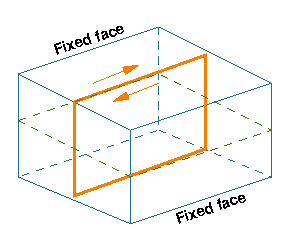
\includegraphics[height=5.0in]{figs/examplehex8}
  \end{center}

% ------------------------------------------------------------ SLIDE
\foilhead{Workflow for Example}
  \summary{}

  \begin{enumerate}
  \item Generate finite-element mesh using CUBIT (hex8 cells)
  \item Create {\tt .cfg} file with simulation parameters
  \item Create containers for materials, boundary conditions, or
    faults (if necessary)
  \item Create spatial database files with parameters for boundary
    conditions and faults
  \item Run pylith
  \item Visualize results with ParaView
  \end{enumerate}

% ------------------------------------------------------------ SLIDE
\foilhead{Useful Tips/Tricks}
  \summary{}

  \begin{itemize}
  \item Command line arguments
    \begin{itemize}
    \item {\tt --help}
    \item {\tt --help-components}
    \item {\tt --help-properties}
    \item {\tt --petsc.start\_in\_debugger} (run in xterm)
    \item {\tt --nodes=N} (to run on N processors on local machine;
      not fully tested)
    \end{itemize}
  \item PyLith 1.0 User Manual
  \item CIG Short-Term Tectonics mailing list
    \begin{itemize}
    \item {\tt cig-short@geodynamics.org}
    \end{itemize}
  \item CIG bug tracking system
    \begin{itemize}
    \item {\tt http://www.geodynamics.org/roundup}
    \end{itemize}
  \end{itemize}

% ------------------------------------------------------------ SLIDE
\foilhead{Feedback}
  \summary{We want your comments!}

  \begin{itemize}
  \item PyLith 1.0 versus PyLith 0.8
    \begin{itemize}
    \item Help prioritize adding features present in PyLith 0.8
    \end{itemize}
  \item PyLith 1.0 versus other codes
    \begin{itemize}
    \item You would like to be using PyLith, but \ldots
    \end{itemize}
  \item PyLith is designed to be a community code
    \begin{itemize}
    \item Contribute bulk constitutive models
    \item Contribute mesh importers
    \item Contribute visualization exporters
    \end{itemize}
  \end{itemize}


% --------------------------------------------------------- DOCUMENT
\end{document}


% End of file
